\documentclass[10pt,nofootinbib,letterpaper]{revtex4}
%\usepackage[nocap]{ctex}

\usepackage{xeCJK}
% if \usrpackage{xetex} it will invoke the open source Fandol Song Font by default, which lack many Chinese characters
% Linux Requires TrueType Fonts from Windows (locating at C:\Windows\Fonts), and Simlink 
% ln -s blablabla /usr/share/fonts/WindowsFonts 
\setCJKmainfont[BoldFont={SimHei},ItalicFont={KaiTi}]{SimSun}
\setCJKfamilyfont{kaishu}{KaiTi} 
\newcommand*{\kaishu}{\CJKfamily{kaishu}}


\usepackage{amsmath,amssymb,amsfonts,mathrsfs,bm,dsfont}
\usepackage{slashed}
\usepackage{enumerate}
\usepackage{enumitem} % Customize itemize, see https://ctan.org/tex-archive/macros/latex/contrib/enumitem/
\usepackage[all]{xy}
\usepackage[noabbrev]{cleveref} % multiple equation ref, see https://tex.stackexchange.com/questions/314217/how-i-can-refer-multiple-equation-in-latex?rq=1
\usepackage[normalem]{ulem}	% delete line
\usepackage{array}
\usepackage{graphics,color}
\usepackage{tikz}
	\usetikzlibrary{calc}
	\usetikzlibrary{decorations.markings}
	\usetikzlibrary{arrows}
	\usetikzlibrary{patterns}
	%\usetikzlibrary{shapes.callouts}
\tikzset{
    level/.style = {
        ultra thick,
        blue,
    },
    connect/.style = {
        dashed,
        red
    },
    label/.style = {
        text width=2cm
    }
}
\usepackage{pgfplots}
%\usepackage[citestyle=authortitle]{biblatex} % able to cite the title, author and year
%\usepackage{hyperref}
\usepackage{feynmp} % feymann diagram
\usepackage{extarrows}
\usepackage[normalem]{ulem} % 文字划掉(横),与 cite 兼容问题,见 https://tex.stackexchange.com/questions/98222/ulem-incompatibility-with-multiple-entries-in-cite
\usepackage{simpler-wick}


\newcommand*\dd{\mathop{}\!\mathrm{d}}
\newcounter{Claim}[section]
\newenvironment{Claim}[1][]{{\par\normalfont\bfseries \underline{Claim~\stepcounter{Claim}\arabic{Claim}.}~#1~~}}{\par}
\newcounter{Property}[section]
\newenvironment{Property}[1][]{{\par\normalfont\bfseries \underline{Property~\stepcounter{Property}\arabic{Property}.}~#1~~}}{\par}
\newcounter{Proposition}[section]
\newenvironment{Proposition}[1][]{{\par\normalfont\bfseries \underline{Proposition~\stepcounter{Proposition}\arabic{Proposition}.}~#1~~}}{\par}
\newcounter{Theorem}[section]
\newenvironment{Theorem}[1][]{{\par\normalfont\bfseries \underline{Theorem~\stepcounter{Theorem}\arabic{Theorem}.}~#1~~}}{\par}
\newcounter{Note}[section]
\newenvironment{Note}[1][]{{\par\normalfont\bfseries \underline{Note~\stepcounter{Note}\arabic{Note}.}~#1~~}}{\par}
\newcounter{Lemma}[section]
\newenvironment{Lemma}[1][]{{\par\normalfont\bfseries \underline{Lemma~\stepcounter{Lemma}\arabic{Lemma}.}~#1~~}}{\par}
\newcounter{Corollary}[section]
\newenvironment{Corollary}[1][]{{\par\normalfont\bfseries \underline{Corollary~\stepcounter{Corollary}\arabic{Corollary}.}~#1~~}}{\par}
\newenvironment{Proof}{{\par~{\normalfont\bfseries $\vartriangleright$}~~}}{\hfill $\square$\par\hfill\par} %\par
\newcounter{Def}[section]
\newenvironment{Def}[1][]{{\par\normalfont\bfseries \underline{Definition~\stepcounter{Def}\arabic{Def}.}~#1~~}}{\par}
\newcounter{Assumption}[section]
\newenvironment{Assumption}[1][]{{\par\normalfont\bfseries \underline{Assumption~\stepcounter{Assumption}\arabic{Assumption}.}~#1~~}}{\par}



\allowdisplaybreaks[4] %允许 align 跨页编排

%\def\checkmark{\tikz\fill[scale=0.4](0,.35) -- (.25,0) -- (1,.7) -- (.25,.15) -- cycle;}
%\def\G{\mathcal{G}}
\def\Z{\mathcal{Z}}
\def\H{\mathcal{H}}
\def\D{\mathcal{D}}

\begin{document}
\title{Linear Response Theory: Two Regimes, Two Parts of Electrical Conductivities, and Many Equivalent Forms of the Adiabatic Response}
\author{Xiaodong Hu}

%\altaffiliation[Also at ]{Boson College}
\email{xiaodong.hu@bc.edu}
\affiliation{Department of Physics, Boston College}

\date{\today}

\begin{abstract}
	In this letter, we will review the general theory of isothermal linear response and adiabatic linear response. Taking adiabatic charge current response as one example, we will show that the standard form of the conductivity tensor, consisting of paramagnetic and diamagnetic parts, can also be obtained by coupling with electrical potentials. We discuss the cancellation of diamagnetic part, and obtain Drude weight in the uniform limit. We also derive some other useful forms of Kubo formula for future reference.\par
	%\begin{center}
		\hfill\par
		{\centering\kaishu 当时共客长安,似二陆初来俱少年。有笔头千字,胸中万卷;致君尧舜,此事何难?\\[0.5em]}
	%\end{center}
	\hfill------ 苏轼「沁园春」
\end{abstract}

\maketitle
\tableofcontents

\section{Linear Response Theory}
	The problem of linear-reponse is formulated as following:\par
	Consider an system in equilibrium coupling with external driven forces through a perturbative fields $F(t)$ (switching on from $t_0$, for example)
	\begin{equation}\label{1.0.1}
		\hat H=\hat H_0+\hat H'(t)\equiv \hat H_0+F(t)\hat B(t),
	\end{equation}
	then for small fields $F(t)$, the meseasurable quantum average of the operator (in Schr\"{o}dinger picture, for example)
	\begin{equation}\label{1.0.2}
		\langle A\rangle(t)\equiv\dfrac{1}{\Z}\mathrm{Tr}\{\hat{\rho}_S(t)\hat A\}\equiv\dfrac{1}{\Z}\sum_{\psi}\langle\psi_S(t)|\hat\rho_S(t)\hat A|\psi_S(t)\rangle
	\end{equation}
	can be expand to the first order of $F(t)$, which is believed to reflect the intrinsic properties of the material. However, depending on the treatment of the perturbation in \eqref{1.0.2}, or more precisely whether we are in the \emph{fast} or \emph{slow} limit\footnote{Following \cite{luttinger1964theory}, the perturbation is fast if the density matrix can be taken as the one in old equilibrium, while is slow if the system is always in (new) quasi-equilibrium.}, we will fall into two regimes --- the (usual) \emph{adiabatic responses} and \emph{isothermal responses}.
	
	\subsection{Isothermal Response}
		For isothermal reponses, the perturbation is \emph{slow} enough so that the system is always in quasi-equilibirum. So we can directly write down
		\begin{equation}\label{1.1.1}
			\hat\rho(t)=\dfrac{1}{\Z}e^{-\beta\hat H}=\dfrac{1}{\Z}e^{-\beta(\hat H_0+\hat H'(t))}.
		\end{equation}
		But even the density matrix is known, it is still hard to expand to the first order of $F(t)$ and evaluate the quantum average for \eqref{1.0.2}. Following \cite{levy2000magnetism}, we can make use of the analogy of imaginary-time and inverse-temperature to define a function of $\beta$ as
		\begin{equation*}
			V(\beta)\equiv e^{-\beta\hat H}e^{\beta\hat H_0}= e^{-\beta(\hat H_0+\hat H'(t))}e^{\beta\hat H_0}.
		\end{equation*}
		Clearly we have
		\begin{align*}
			\dfrac{\dd V(\beta)}{\dd\beta}&=e^{-\beta\hat H(t)}\hat H_0 e^{\beta\hat H_0}-e^{-\beta\hat H(t)}\hat H(t)e^{\beta\hat H_0}\equiv e^{-\beta\hat H(t)}\hat H'(t)e^{\beta\hat H_0}\\
			&\equiv e^{-\beta\hat H(t)}e^{\beta\hat H_0}\cdot e^{-\beta\hat H_0}\hat H'(t)e^{\beta\hat H_0}\equiv V(\beta)\hat H'_I(t+i\hbar\beta),
		\end{align*}
		where $\hat H'_I(t+i\hbar\lambda)\equiv F(t)\hat B(i\hbar\lambda)$. This differential equation is equivalent to the integral equation (check by differentiation)
		\begin{equation}\label{1.1.2}
			V(\beta)=1+\int_0^\beta\dd\lambda\,V(\lambda)\hat H'_I(t+i\hbar\lambda),
		\end{equation}
		which can be solved iteratively. To the first-order approximation, we can take $\hat H'(t)=0$ in the definition of $V(\beta)$ (so to the zeroth order $V(\beta)=1$), getting
		\begin{equation}\label{1.1.3}
			V(\beta)\simeq1+\int_0^\beta\dd\lambda\,\hat H'_I(t+i\hbar\lambda)
		\end{equation}
		So
		\begin{equation}\label{1.1.4}
			e^{-\beta\hat H(t)}\equiv V(\beta)e^{-\beta\hat H_0}\simeq \left(1+\int_0^\beta\dd\lambda\,\hat H'_I(t+i\hbar\lambda)\right)e^{-\beta\hat H_0} 
		\end{equation}
		and the variation of the quantum average of the operator $\hat A$ takes the form of
		\begin{equation}\label{1.1.5}
			\delta \langle\hat A\rangle=\dfrac{1}{\Z}\mathrm{Tr}\{e^{-\beta\hat H(t)}\hat A\}-\dfrac{1}{\Z}\mathrm{Tr}\{e^{-\beta\hat H_0}\hat A\}=\int_0^\beta\dd\lambda\,\langle\hat A\hat H'_I(t+i\hbar\lambda)\rangle_0=\int_0^\beta\dd\lambda \langle\hat A e^{-\beta\hat H_0}\hat B e^{\beta\hat H_0}\rangle F(t).
		\end{equation}
		The \emph{isothermal response}
		\begin{equation}\label{1.1.6}
			\chi_{AB}^T\equiv\int_0^\beta\dd\lambda\,\langle\hat A e^{-\lambda\hat H_0}\hat Be^{\lambda\hat H_0}\rangle
		\end{equation}
		 can be easily expressed in the energy basis: splitting into the cases when $m\neq n$ and $m=n$ and perform the integral over inverse-temperature, we have
		 \begin{equation}\label{1.1.7}
		 	\chi_{AB}^T=\sum_{m,n}\int_0^\beta\dd\lambda\,e^{-\beta \varepsilon_n}A_{nm}e^{-\lambda \varepsilon_m}B_{mn}e^{-\lambda \varepsilon_n}=\sum_{\substack{m,n\\m\neq n}}A_{nm}B_{mn}\dfrac{e^{-\beta \varepsilon_m}-e^{-\beta \varepsilon_n}}{\varepsilon_n- \varepsilon_m}-\beta\sum_n e^{-\beta \varepsilon_n}A_{nn}B_{nn}.
		 \end{equation}
		 
	\subsection{Adiabatic Response}
		For the more widely-used adiabatic responses, however, \textbf{we have no assumption on the form of the time-dependent density matrix, but can only determine it from the definition}
		\begin{equation}\label{1.2.1}
			\dot{\hat\rho}_S(t)=\dfrac{1}{i\hbar}[\hat H_0+\hat H'(t),\hat\rho_S(t)].
		\end{equation}
		\begin{Note}
			There are some literatures\footnote{Like Sec. 3.2.1 of \cite{giuliani2005quantum} and Sec. 8.3 of \cite{levy2000magnetism}.} going that the characteristic of the adiabatic response is that the density matrix can be assumed to stay as the same one in the old equilibrium $\hat\rho(t)=e^{-\beta\hat H_0}/\Z$ so that all-time dependence of adiabatic responses original from the time-evolved states. Such claim is true at least for linear response (giving the same result), but I am not sure if this is true for non-linear response as well. So I would not address in this way.
		\end{Note}
		\hfill\par
		To solve the Liuville equation \eqref{1.2.1}, it is helpful to switch into the interaction picture $\hat\rho_I(t)\equiv U_0^{-1}(t)\hat\rho_S(t)U_0(t)\equiv e^{\frac{i}{\hbar}\hat H_0t}\hat\rho_S(t)e^{-\frac{i}{\hbar}\hat H_0t}$, leaving
		\begin{equation}\label{1.2.2}
			\dot{\hat\rho}_I(t)=\dfrac{1}{i\hbar}U_0^{-1}(t)[\hat H'(t),U_0(t)\hat\rho_I(t)U_0^{-1}(t)]U_0(t)=\dfrac{1}{i\hbar}[\hat H'_I(t),\hat\rho_I(t)]\equiv \hat L_I'\hat\rho_I(t),
		\end{equation}
		where the interaction picture operator $\hat H_I'(t)\equiv U_0^{-1}(t)\hat H'(t)U_0(t)\equiv e^{\frac{i}{\hbar}\hat H_0t}\hat H'(t)e^{-\frac{i}{\hbar}\hat H_0t}$ and we introduce a Liouville operator $\hat L'_I\hat{\mathcal{O}}:=\frac{1}{i\hbar}[\hat H'_I,\hat{\mathcal{O}}]$.\par
		Differential equation \eqref{1.2.2} can be solved iteratetively: the zeroth-order solution is just the old equilibrium density matirix $\hat\rho_I(t_0)\equiv\hat\rho_S(t_0)\equiv\rho_0$, the first-order solution is obtained by inserting $\hat\rho_0$ into \eqref{1.2.2}, the second order is obtained by inserting the first-order, and so on. Namely, $\hat\rho_I(t)$ can be expressed in terms of \emph{Dyson series}
		\begin{align}
			\hat\rho_I(t)&=\hat\rho_0+\dfrac{1}{i\hbar}\int_{t_0}^t\dd\tau\,\hat L_I'(\tau)\hat\rho_0+\left(\dfrac{1}{i\hbar}\right)^2\int_{t_0}^t\dd\tau_2\int_{t_0}^{\tau_2}\dd\tau_1\,\hat L_I'(\tau_2)\hat L_I'(\tau_1)\hat\rho_0+\cdots.\nonumber\\
			&=\hat\rho_0+\dfrac{1}{i\hbar}\int_{t_0}^t\dd\tau\,[\hat H'_I(\tau),\hat\rho_0]+\left(\dfrac{1}{i\hbar}\right)^2\int_{t_0}^t\dd\tau_2\int_{t_0}^{\tau_2}\dd\tau_1\,[\hat H'_I(\tau_2),[\hat H'_I(\tau_1),\hat\rho_0]]+\cdots.\label{1.2.3}
		\end{align}
		Therefore, the evaluation of \eqref{1.0.2} can be done in the interaction picture by cycling the trace
		\begin{align}
			\langle\hat A\rangle(t)&\equiv\mathrm{Tr}\{\hat\rho_S(t)\hat A_S\}=\mathrm{Tr}\{\hat\rho_I(t)e^{\frac{i}{\hbar}H_0 t}\hat A_Se^{-\frac{i}{\hbar}H_0t}\}\equiv\mathrm{Tr}\{\rho_I(t)\hat A_I(t)\}\nonumber\\
			&=\mathrm{Tr}\{\hat\rho_0\hat A_I(t)\}+\dfrac{1}{i\hbar}\int_{t_0}^t\dd\tau\,\mathrm{Tr}\{[\hat H'_I(\tau),\hat\rho_0]\hat A_I(t)\}+\left(\dfrac{1}{i\hbar}\right)^2\int_{t_0}^t\dd\tau_2\int_{t_0}^{\tau_2}\dd\tau_1\,\mathrm{Tr}\bigg\{[\hat H'_I(\tau_2),[\hat H'_I(\tau_1),\hat\rho_0]]\hat A_I(t)\bigg\}+\cdots\nonumber\\
			&=\langle\hat A\rangle_0+\dfrac{1}{i\hbar}\int_{t_0}^t\dd\tau\,\langle[\hat A_I(t),\hat H'_I(\tau)]\rangle_0+\left(\dfrac{1}{i\hbar}\right)^2\int_{t_0}^t\dd\tau_2\int_{t_0}^{t_2}\dd\tau_1\,\langle [[\hat A_I(t),\hat H'(\tau_2)],\hat H'_I(\tau_1)]\rangle_0+\cdots,\label{1.2.4}
		\end{align}
		where the first term (equilibrium average) is vanishing due to Bloch's theorem, and for the other terms identity
		\begin{equation*}
			\mathrm{Tr}\{[A,B]C\}\equiv\mathrm{Tr}\{B[C,A]\}.
		\end{equation*}
		is used to take out $\hat\rho_0$ and recover the quantum average. Without loss of generality, from now on we take $t_0\rightarrow-\infty$.\par
		\hfill\par

		If $\hat H'(t)$ is introduced in the way of \eqref{1.0.1}, the linear response is
		\begin{equation}\label{1.2.5}
			{\color{red}\delta \langle\hat A\rangle^{(1)}(t)=\dfrac{1}{i\hbar}\int_{-\infty}^t\dd t'\,\langle[\hat A_I(t),\hat B_I(t')]\rangle_0\cdot F(t'),}
		\end{equation}
		or in terms of \emph{retarded} Green function
		\begin{equation}\label{1.2.6}
			\delta \langle\hat A\rangle^{(1)}(t)=\dfrac{1}{\hbar}\int_{-\infty}^\infty\dd t' G_{AB}^R(t,t')F(t'),\quad G_{AB}^R(t,t')=(-i)\theta(t-t')\langle[\hat A_I(t),\hat B_I(t')]\rangle_0
		\end{equation}
		if the integral \eqref{1.2.5} is extended to the entire domain of time. 
		\begin{Note}
			Comparing \eqref{1.2.5} with \eqref{1.1.5}, the most intuitive difference of isothermal response function and adiabatic response function is that the former one does not depend on time! This is resonable since the time-evolution of isothermal processes cannot be perceived by the system (it is always in quasi-equilibrium). 
		\end{Note}
		\hfill\par
		Note that by cycling the time arguments of operator $\hat A$ and $\hat B$ in the retarded Green function, $G_{AB}^R(t,t')\equiv G^R_{AB}(t-t',0)$ so the R.H.S. of \eqref{1.2.6} has exactly the form of a \emph{convolution}. According to convolution theorem\footnote{The Fourier transformation of a convolution of two functions is the multiplication of each's Fourier transformation.}, we have, in frequency domain,
		\begin{equation}\label{1.2.7}
			\delta\langle\hat A\rangle(\omega)=\chi_{AB}(\omega)F(\omega),
		\end{equation}
		where
		\begin{equation}\label{1.2.8}
			 {\color{red}\chi_{AB}(\omega)\equiv\mathbb{F}\left[\dfrac{1}{\hbar}G_{AB}^R(t,0)\right]\equiv\lim_{s \rightarrow0^+}\dfrac{1}{\hbar}G_{AB}^R(\varpi)=\lim_{s\rightarrow0^+}\dfrac{1}{i\hbar}\int_0^\infty\dd t\,\langle[\hat A_I(t),B_I]\rangle_0 e^{i\varpi t}},
		\end{equation}
		where an infinitesimal positive number is inserted $\varpi\equiv\omega+is$ because the retarded function $G_{AB}^R(\varpi)$ is analytical only on the upper-half plane of the frequency domain \cite{abrikosov2012methods}. Another thing that needs to keep in mind is that unlike the integration domain in time space in \eqref{1.2.6}, for response function in frequency space the integration is taken within $[0,+\infty)$.\par
		Morever, if the system remains translation-invariant (this happens at least when we concern about only long wave-length physics) $\chi_{AB}(\bm{r},\bm{r'};\omega)\equiv\chi_{AB}(\bm{r}-\bm{r'};\omega)$, the response function in momentum space
		\begin{equation*}
			\langle\hat A\rangle(\bm{q},\omega)=\chi_{AB}(\bm{q},\omega)F(\omega)
		\end{equation*}
		reads
		\begin{equation}\label{1.2.9}
			\chi_{AB}(\bm{q},\omega)=\lim_{s \rightarrow0^+}\dfrac{1}{i\hbar V}\int_0^\infty\dd t\,\langle[\hat A_I(\bm{q},t),\hat B_I(\bm{-q},0)]\rangle_0 e^{i\varpi t}.
		\end{equation}
		This is because (taking Fourier transformation to second-quantized operators)
		\begin{align*}
			\chi_{AB}(\bm{r},\bm{r'};\omega)&\equiv\lim_{s \rightarrow0^+}\dfrac{1}{i\hbar V}\int_0^\infty\dd t\,\sum_{\bm{k},\bm{k'}} e^{i\bm{k}\cdot\bm{r}}e^{i\bm{k'}\cdot\bm{r'}}\langle[\hat A_I(\bm{k},t),\hat B_I(\bm{k'},0)]\rangle_0 e^{i\varpi t}\\
			&\equiv\lim_{s \rightarrow0^+}\dfrac{1}{i\hbar V}\int_0^\infty\dd t\,\sum_{\bm{k},\bm{k'}} e^{i\bm{k}\cdot(\bm{r}-\bm{r'})}e^{i(\bm{k}+\bm{k'})\cdot\bm{r'}}\langle[\hat A_I(\bm{k},t),\hat B_I(\bm{k'},0)]\rangle_0 e^{i\varpi t}.
		\end{align*}
		is a function of $\bm{r}-\bm{r'}$ if and only if $\bm{k}+\bm{k'}\equiv0$.\par
		In the energy eigenstate, the response function takes the form of
		\begin{align}
			\chi_{AB}(\omega)&=\lim_{s\rightarrow0^+}\dfrac{1}{i\hbar}\int_0^\infty\dd\tau\,\sum_{m,n}(e^{-\beta \varepsilon_n}-e^{-\beta \varepsilon_m})A_{nm}B_{mn}e^{\frac{i}{\hbar}(\varepsilon_n- \varepsilon_m)\tau} e^{i(\omega+is)\tau}\nonumber\\
			&=\lim_{s\rightarrow0^+}\sum_{m,n}\dfrac{e^{-\beta \varepsilon_n}-e^{-\beta \varepsilon_m}}{\hbar\omega+\varepsilon_n- \varepsilon_m+is}A_{nm}B_{mn}.\label{1.2.10}
		\end{align}
		Comparing with \eqref{1.1.7}, this time the denomenator is always well-defined so we do not have to split into the diagonal and off-diagonal parts before performing the integral.
		\begin{Note}
			The off-diagonal part of isothermal response \eqref{1.1.7} is clear to coincides with the static limit of adiabatic response $\displaystyle\lim_{\omega\rightarrow0}\chi_{AB}(\omega)$, while the diagonal part of \eqref{1.1.7} is exclusive. Anyway \textbf{in general isothermal responses do not have to be the same as the static limit of adiabatic responses --- they are two quite different things.}
		\end{Note}

	\subsection{Example: Adiabatic Response of Charge Current}
		In this section, we will consider the electric current driven by an external electric field. In general such electric field depends on both scalar and vector potentials
		\begin{equation*}
			\bm{E}(\bm{r},t)\equiv-\nabla\phi-\dfrac{\partial\bm{A}}{\partial t}.
		\end{equation*}
		Under the minimal coupling with external vector potential, the general continuum Hamiltonian with impurity potentials $V_{\text{imp}}$ and interacting terms $U$ (like four-fermion Coulomb interaction)
		\begin{equation}\label{1.3.1}
			H=\int\dd\bm{r}\,\psi^\dagger(\bm{r},t)\bigg(-\dfrac{\hbar^2}{2m}\nabla^2-\mu+V_{\text{imp}}(\bm{r})\bigg)\psi(\bm{r},t)+U
		\end{equation}
		becomes (we work in SI units so $A^\mu=(\frac{\phi}{c},\bm{A})$)
		\begin{align}
			H[A_\mu]&=\int\dd\bm{r}\,\psi^\dagger(\bm{r},t)\left(\dfrac{1}{2m}\left(\dfrac{\hbar}{i}\nabla-q\bm{A}(\bm{r},t)\right)^2+\dfrac{q}{c}\phi(\bm{r},t)-\mu+V_{\text{imp}}\right)\psi(\bm{r},t)+U\nonumber\\
			&=H[0]-\dfrac{q\hbar}{2im}\int\dd\bm{r}\,\bigg(\psi^\dagger(\bm{r},t)\bm{A}(\bm{r},t)\cdot\nabla\psi(\bm{r},t)-\nabla\psi^\dagger(\bm{r},t)\cdot\bm{A}(\bm{r},t)\psi(\bm{r},t)\bigg)\nonumber\\
			&\qquad+\dfrac{q}{c}\int\dd\bm{r}\,\psi^\dagger(\bm{r},t)\phi(\bm{r},t)\psi(\bm{r},t)+\dfrac{q^2}{2m}\int\dd\bm{r}\,\psi^\dagger(\bm{r})\bm{A}(\bm{r},t)^2\psi(\bm{r}).\label{1.3.2}
		\end{align}
		By definition of charge current $J_\mu\equiv\dfrac{\delta S[A_\mu]}{\delta A_\mu}$, we get, in the metric $\dd s^2=-c^2\dd t^2+\dd\bm{x}^2$
		\begin{equation}\label{1.3.5}
			H[A_\mu]=H[0]-\bm{J}\cdot\bm{A}+A_0J^0,
		\end{equation}
		where
		\begin{align}
			J^0(\bm{r},t)&\equiv\dfrac{\delta H[A_\mu]}{\delta A_0}=\dfrac{\delta H}{\delta(\phi/c)}=q\psi^\dagger(\bm{r},t)\psi(\bm{r},t),\label{1.3.3}\\
			J^i(\bm{r},t)&\equiv-\dfrac{\delta H[A_\mu]}{\delta A_i}=\dfrac{q\hbar}{2im}\bigg(\psi^\dagger(\bm{r},t)(\partial^i\psi(\bm{r},t))-(\partial^i\psi^\dagger(\bm{r},t))\psi(\bm{r},t)\bigg)-\dfrac{q^2}{m}\psi^\dagger(\bm{r},t)A^i(\bm{r},t)\psi(\bm{r},t)=:J^{P,i}(\bm{r},t)+J^{D,i}(\bm{r},t),\label{1.3.4}
		\end{align}
		where we introduce the \emph{paramagnetic} part $\bm{J}^P$ (of order $\mathcal{O}((A_\mu)^0)$) and \emph{diamagnetic} part $\bm{J}^D$ (of order $\mathcal{O}(A_\mu)$) of the charge current.\par
		Keeping track of merely \emph{linear} coupling of the Hamiltonian, i.e., separating the contribution of paramagnetic and diamagnetic parts in consideration of adabatic linear response, we can make use of the general result of adabatic linear response to write down the quantum average of total current at time $t$ as
		\begin{align}
			\langle J_\alpha(\bm{r},t)\rangle^{(1)}&=\langle J_\alpha^P(\bm{r},t)\rangle^{(1)}-\dfrac{q^2}{m}\langle\psi^\dagger(\bm{r},t)\psi(\bm{r},t)\rangle^{(0)}A_\alpha(\bm{r},t)(1-\delta_{\alpha0})\nonumber\\
			&=\dfrac{-1}{i\hbar}\int_{-\infty}^0\dd t'\int\dd\bm{r'}\,\langle[J^P_{\alpha,I}(\bm{r},t),J^P_{\beta,I}(\bm{r'},t')]\rangle_0 A_\beta(\bm{r'},t)-\dfrac{q^2}{m}n_0(1-\delta_{\alpha0})A_\alpha(\bm{r},t)\nonumber\\
			&=\int\dd\bm{r'}\int\dd t'\,\bigg\{\dfrac{-1}{i\hbar}\theta(t-t')\langle[J^P_{\alpha,I}(\bm{r},t),J^P_{\beta,I}(\bm{r'},t')]\rangle_0-\dfrac{q^2}{m}n_0\delta_{\alpha\beta}(1-\delta_{\alpha0})\delta(\bm{r}-\bm{r'})\delta(t-t')+\bigg\}A^{\beta}(\bm{r'},t'),\label{1.3.6}
		\end{align}
		where in the first line we take the zeroth-order approximation for the diamagnetic part so that the particle density remains to be spacetime-independent $n(\bm{r},t)\equiv\langle\psi^\dagger(\bm{r},t)\psi(\bm{r},t)\rangle=n_0$ as the one in the old equilibrium (note that spacetime-fluctuation is all brought by the external stimulus). The extra minus sign for the adiabatic response of paramagnetic currents in the second line comes from the negative coupling with external vector potential (see \eqref{1.3.5}).\par
		Since the expression in the curly brace in \eqref{1.3.6} is still a function of $t-t'$, then convolution theorem tells
		\begin{equation}\label{1.3.7}
			\langle J_\alpha(\bm{r},\omega)\rangle^{(1)}=\int\dd\bm{r'}\sigma_{\alpha\beta}(\bm{r},\bm{r'};\omega)E_\beta(\bm{r'},\omega),
		\end{equation}
		with the conductivity matrix
		\begin{equation}\label{1.3.8}
			\sigma_{\alpha\beta}(\bm{r},\bm{r'};\omega)=\dfrac{-1}{i\omega}\left[\chi_{\alpha\beta}^P+\dfrac{q^2}{m}n_0\delta_{\alpha\beta}(1-\delta_{\alpha0})\delta(\bm{r}-\bm{r'})\right],\quad\chi_{\alpha\beta}^P\equiv\lim_{s\rightarrow0^+}\dfrac{1}{i\hbar}\int_0^\infty\dd t\,\langle[J^P_{\alpha,I}(\bm{r},t),J^P_{\beta,I}(\bm{r'},0)]\rangle_0 e^{i\varpi t},
		\end{equation}
		where we take the gauge $\phi=0$ and express the electric field in terms of the vector potential $\bm{E}(\omega)=i\omega\bm{A}(\omega)$ in the frequency domain. Such step of gauge fixing can be done at the very beginning to simplify the form of the current operator (by setting $J^0=0$).\par
		Anyway, if the material is furthermore homogeneous $\sigma_{\alpha\beta}(\bm{r},\bm{r'};\omega)\equiv\sigma_{\alpha\beta}(\bm{r}-\bm{r'};\omega)$, we have
		\begin{equation}\label{1.3.9}
			\langle J_\alpha(\bm{q},\omega)\rangle^{(1)}=\dfrac{-1}{i\omega}\left\{\chi^P_{\alpha\beta}(\bm{q},\omega)+\dfrac{q^2}{m}n_0\delta_{\alpha\beta}(1-\delta_{\alpha0})\right\}E^\beta(\bm{q},\omega),
		\end{equation}
		with the paramagnetic response function
		\begin{equation}\label{1.3.10}
			\quad\chi_{\alpha\beta}^P(\bm{q},\omega)\equiv\lim_{s\rightarrow0^+}\dfrac{1}{i\hbar V}\int_0^\infty\dd t\,\langle[J^P_{\alpha,I}(\bm{q},t),J^P_{\beta,I}(-\bm{q},0)]\rangle_0 e^{i\varpi t}.
		\end{equation}
	
	\subsection{Drude Formula: Cancellation of Static Diamagnetic Response in Metals}
		DC limit (\emph{slow limit}) of conductivity is taken in the order of
		\begin{equation}\label{1.4.1}
			\sigma_{\alpha\beta}^{\text{DC}}:=\lim_{\omega \rightarrow0}\lim_{\bm{q}\rightarrow0}\sigma_{\alpha\beta}(\bm{q},\omega).
		\end{equation}
		A first glance of \eqref{1.3.9} tells that there is a divergence provided $\chi_{\alpha\beta}(\bm{q},\omega)$ was analytic, conflicting with the physical observations for large amounts of materials. However, we will show below that for band metals (where only intra-band processes dominate) such divergence is exactly cancelled by the term containing in the paramagnetic part. Denoting $I_{\alpha\beta}(t)\equiv\langle\hat J_\alpha(t)\hat J_\beta\rangle_0$ and expressiong the many-body current operator as a summation of single-particle current operator $\hat J_\alpha=\sum_{\mu\nu}\langle\mu|J^{(1)}_\alpha|\nu\rangle \hat a_\mu^\dagger\hat a_\nu$, we have (only \emph{connected} diagram contributes\footnote{This fact is much clearer in path-integral formalism, see, for example, \cite{fradkin2013field}.})
		\begin{align*}
			I_{\alpha\beta}(t)-I_{\beta\alpha}(t)&=\sum_{1,2,3,4}\wick{\bigg\langle\langle 1|J^{(1)}_\alpha|2\rangle\c1 a_1^\dagger(t) \c2 a_2(t)\langle 3|J^{(1)}_\beta|4\rangle \c2 a_3^\dagger \c1 a_4\bigg\rangle-(\alpha\leftrightarrow\beta)}\\
			&=\sum_{1,2,3,4}\langle 1|J^{(1)}_\alpha|2\rangle\langle 3|J^{(1)}_\beta|4\rangle\left\langle 4\middle|\dfrac{e^{\frac{i}{\hbar}ht}}{1+e^{\beta h}}\middle|1\right\rangle\left\langle2\middle|\dfrac{e^{-\frac{i}{\hbar}ht}}{1+e^{-\beta h}}\middle|3\right\rangle-(\alpha\leftrightarrow\beta)\\
			&=\sum_{m,n}e^{\frac{i}{\hbar}(\varepsilon_m-\varepsilon_n)t}\langle m|J^{(1)}_\alpha|n\rangle\langle n|J^{(1)}_\beta|m\rangle\left[\dfrac{1}{1+e^{\beta \varepsilon_m}}\dfrac{e^{\beta \varepsilon_n}}{1+e^{\beta \varepsilon_n}}-\dfrac{e^{\beta \varepsilon_m}}{1+e^{\beta \varepsilon_m}}\dfrac{1}{1+e^{\beta \varepsilon_n}}\right]\\
			&=\sum_{m,n}e^{\frac i\hbar(\varepsilon_m-\varepsilon_n)t}\langle m|J^{(1)}_\alpha|n\rangle\langle n|J^{(1)}_\beta|m\rangle(f_m-f_n),
		\end{align*}
		where in the second line we use, for free fermion $\hat H_0=\sum_{\alpha\beta}c_\alpha^\dagger h_{\alpha\beta}c_\beta$,
		\begin{align*}
			\langle c_\alpha^\dagger(t)c_\beta\rangle&\equiv\left\langle e^{-\frac i\hbar\hat H_0 t} c_\alpha^\dagger e^{\frac i\hbar\hat H_0 t}c_\beta\right\rangle=\bigg\langle\bigg(c_\alpha^\dagger-i\frac t\hbar[\hat H_0,c_\alpha^\dagger]+\dfrac{t^2}{(2\hbar)!}[\hat H_0,[\hat H_0,c_\alpha^\dagger]]+\cdots\bigg)c_\beta\bigg\rangle\\
			&=\sum_\gamma\left(e^{\frac i\hbar ht}\right)_{\gamma\alpha}\langle c_\gamma^\dagger c_\beta\rangle=\left\langle \beta\middle|\dfrac{e^{\frac i\hbar ht}}{1+e^{\beta h}}\middle|\alpha\right\rangle,
		\end{align*}
		and similarly
		\begin{equation*}
			\langle c_\alpha(t)c_\beta^\dagger\rangle=\sum_\gamma\left(e^{-\frac i\hbar ht}\right)_{\alpha\gamma}\langle c_\gamma c_\beta^\dagger\rangle=\left\langle \alpha\middle|\dfrac{e^{-\frac i\hbar ht}}{1+e^{\beta h}}\middle|\beta\right\rangle,
		\end{equation*}
		with $h$ the first-quantized (single-particle) Hamiltonian. Thus by integrating out the time, the paramagnetic current-current response function reads
		\begin{equation}\label{1.4.2}
			\chi_{\alpha\beta}^P(\bm{q},\omega)=\lim_{s \rightarrow0^+}\dfrac{1}{i\hbar V}\int_0^\infty\dd t\,(I_{\alpha\beta}(t)-I_{\beta\alpha(t)})e^{i\varpi t}=\lim_{s \rightarrow0^+}\dfrac{1}{V}\sum_{m,n}(f_m-f_n)\dfrac{\langle m|J^{(1)}_\alpha(\bm{q})|n\rangle\langle n|J^{(1)}_\beta(\bm{-\bm{q}})|m\rangle}{\hbar\varpi+\varepsilon_m-\varepsilon_n}.
		\end{equation}
		\indent Re-expression the second-quantized paramagnetic current operator \eqref{1.3.4} as
		\begin{equation*}
			J^P_\alpha=\sum_{\bm{r},\bm{r'}}\psi(\bm{r})^\dagger\dfrac{q}{2m}\bigg(\langle\bm{r}|(-i\hbar\nabla')\bm{r'}\rangle+\langle(-i\hbar\nabla)\bm{r}|\bm{r'}\rangle\bigg)\psi(\bm{r'}),
		\end{equation*}
		the single-particle current operator $J^{(1)}_\alpha$ in the coordinate representation $\hat J_\alpha=\sum_{\bm{r},\bm{r'}} \langle\bm{r}|J^{(1)}_{\alpha}|\bm{r'}\rangle\psi_{\bm{r}}^\dagger\psi_{\bm{r'}}$ can be directly read out
		\begin{equation}\label{1.4.3}
			J^{(1)}_\alpha(\bm{r})=\dfrac{q}{2m}(\hat p_\alpha\delta(\bm{r}-\hat{\bm{r}})+\delta(\bm{r}-\hat{\bm{r}})\hat{p}_\alpha),
		\end{equation}
		or in momentum representation
		\begin{equation}\label{1.4.4}
			J^{(1)}_\alpha(\bm{q})=\dfrac{q}{2m}(\hat p_\alpha e^{-\frac i\hbar\bm{q}\cdot\hat{\bm{r}}}+e^{-\frac i\hbar\bm{q}\cdot\hat{\bm{r}}}\hat{p}_\alpha).
		\end{equation}
		Separating the denomenator of equation \eqref{1.4.2} into two parts, we get
		\begin{align}
			\chi_{\alpha\beta}^P(\bm{q},\omega)&=\lim_{s \rightarrow0^+}\dfrac{1}{V}\sum_{m,n}(f_m-f_n)\dfrac{\langle m|J^{(1)}_\alpha(\bm{q})|n\rangle\langle n|J^{(1)}_\beta(-\bm{q})|m\rangle}{\hbar\varpi+\varepsilon_{mn}}\\
			&\equiv\lim_{s \rightarrow0^+}\dfrac{1}{V}\sum_{m,n}(f_m-f_n)\langle m|J^{(1)}_\alpha(\bm{q})|n\rangle\langle n|J^{(1)}_\beta(-\bm{q})|m\rangle|\left[\dfrac{1}{\varepsilon_{mn}}\left(1-\dfrac{\hbar\varpi}{\hbar\varpi+\varepsilon_{mn}}\right)\right].\label{1.4.5}
		\end{align}
		\indent It is clear that with the help of \emph{f-sum rule} (the proof is given in the appendix)
		\begin{equation}\label{1.4.6}
			{\color{red}\sum_{m,n}(f_m-f_n)\dfrac{\langle m|J^{(1)}_\alpha(\bm{q})|n\rangle\langle n|J^{(1)}_\alpha(-\bm{q})|m\rangle}{\varepsilon_m-\varepsilon_n}=-\frac{Nq^2}{m}\delta_{\alpha\beta}},
		\end{equation}
		the first part of response function
		\begin{equation}\label{1.4.7}
			\chi_{\alpha\beta}^{P,\text{1st}}(\bm{q},\omega)\equiv\lim_{s \rightarrow0^+}\dfrac{1}{V}\sum_{m,n}(f_m-f_n)\dfrac{\langle m|J^{(1)}_\alpha(\bm{q})|n\rangle\langle n|J^{(1)}_\beta(-\bm{q})|m\rangle}{\varepsilon_m-\varepsilon_n}=-\dfrac{q^2 n}{m}\delta_{\alpha\beta}
		\end{equation}
		cancels exactly with the the diamagnetic part in the conductivity tensor \eqref{1.3.8}, leaving only
		\begin{equation}\label{1.4.8}
			{\color{red}\sigma_{\alpha\beta}(\bm{q},\omega)=\dfrac{-1}{i\omega}\chi_{\alpha\beta}^{P,\text{2nd}}=\lim_{s \rightarrow0^+}\dfrac{\hbar}{iV}\sum_{m,n}(f_m-f_n)\dfrac{\langle m|J^{(1)}_\alpha(\bm{q})|n\rangle\langle n|J^{(1)}_\beta(-\bm{q})|m\rangle}{\varepsilon_{mn}(\hbar\varpi+\varepsilon_{mn})}}.
		\end{equation}
		\begin{Note}
			Althought the motivation to think about the diamagnetic cancellation starts by observing an abnormal divergence when taking the the static limit $\omega \rightarrow 0$ of physical responses, the above derivation of cancellation is formally true for the whole energy scale! Even if there is a divergence for some materials like BCS superconductors, it comes from \eqref{1.4.8}.
		\end{Note}
		\hfill\par
		The left task is to evaluate the quantum average within the Bloch states $|n\bm{k}\rangle$. For \textbf{the uniform limit $\bm{q}\rightarrow\bm{0}$ of band metals where intra-band processes dominate}, we get (spin degeneracy included)
		\begin{equation*}
			\sigma_{\alpha\beta}^{\text{intra}}(\bm{q},\omega)=\lim_{s \rightarrow0^+}\dfrac{\hbar q^2}{i4m^2V}\sum_{n,s}\sum_{\bm{k},\bm{k'}}(f_{n\bm{k}}-f_{n\bm{k'}})\dfrac{\langle n\bm{k}|\hat p_\alpha e^{-\frac i\hbar\bm{q}\cdot\hat{\bm{r}}}+e^{-\frac i\hbar\bm{q}\cdot\hat{\bm{r}}}\hat p_\alpha|n\bm{k'}\rangle\langle n\bm{k'}|\hat p_\beta e^{\frac i\hbar\bm{q}\cdot\hat{\bm{r}}}+e^{\frac i\hbar\bm{q}\cdot\hat{\bm{r}}}\hat p_\beta|n\bm{k}\rangle}{(\varepsilon_{n\bm{k}}-\varepsilon_{n\bm{k'}})(\hbar\omega+is+\varepsilon_{n\bm{k}}-\varepsilon_{n\bm{k'}})}.
		\end{equation*}
		Using the definition of Block states $\langle\bm{r}|n\bm{k}\rangle\equiv e^{i\bm{k}\cdot\bm{r}}u_n(\bm{r})$, we have
		\begin{equation*}
			e^{\frac i\hbar\bm{q}\cdot\hat{\bm{r}}}|n\bm{k}\rangle=\int\dd\bm{r}\,e^{\frac i\hbar\bm{q}\cdot\hat{\bm{r}}}|\bm{r}\rangle\langle\bm{r}|n\bm{k}\rangle\equiv\int\dd\bm{r}\,e^{\frac i\hbar\bm{q}\cdot\bm{r}}e^{\frac i\hbar\bm{k}\cdot\bm{r}}u_n(\bm{r})=|n,\bm{k}+\bm{q}\rangle,
		\end{equation*}
		and, for example $\langle n\bm{k}|\hat p_\alpha e^{-\frac i\hbar\bm{q}\cdot\hat{\bm{r}}}|n\bm{k'}\rangle=m\delta_{\bm{k},\bm{k'}-\bm{q}}\langle n\bm{k}|\hat v_\alpha|n\bm{k}\rangle$. Thus the intra-band conductivity
		\begin{equation}\label{1.4.9}
			\sigma_{\alpha\beta}^{\text{intra}}(\bm{q},\omega)=\lim_{s \rightarrow0^+}\dfrac{2\hbar q^2}{iV}\sum_{n,\bm{k}}\dfrac{f_{n,\bm{k}}-f_{n,\bm{k+q}}}{\varepsilon_{n,\bm{k}}-\varepsilon_{n,\bm{k'+q}}}\dfrac{\langle n\bm{k}|\hat v_\alpha|n\bm{k}\rangle \langle n\bm{k}|\hat v_\beta|n\bm{k}\rangle}{\hbar\omega+is+\varepsilon_{n,\bm{k}}-\varepsilon_{n,\bm{k+q}}}.
		\end{equation}
		For quadratic dispersion relation, we have, in the uniform limit,
		\begin{equation}\label{1.4.10}
			\sigma_{\alpha\beta}^{\text{intra}}(\bm{q}\rightarrow\bm{0},\omega)\simeq\lim_{s \rightarrow0^+}\dfrac{2\hbar q^2}{iV}\sum_{n,\bm{k}}\left(\dfrac{\partial f_{n\bm{k}}}{\partial \varepsilon_{n\bm{k}}}\right)\dfrac{\langle n\bm{k}|\hat v_\alpha|n\bm{k}\rangle \langle n\bm{k}|\hat v_\beta|n\bm{k}\rangle}{\hbar\omega+is-\frac{\hbar^2}{m}\bm{k}\cdot\bm{q}}.
		\end{equation}
		Equation \eqref{1.4.10} agrees with the result derived from the Boltzmann equation (if we identify the relaxation time $\tau\sim\hbar/s$). If we further ignore the linear-$\bm{q}$ term in \eqref{1.4.10}, we get ($\eta\equiv s/\hbar\ll 1$)
		\begin{equation}\label{1.4.11}
			\sigma_{\alpha\beta}^{\text{intra}}(\bm{q}\rightarrow\bm{0},\omega)\simeq\lim_{\eta \rightarrow0^+}\dfrac{i}{\omega+i\eta}\times\dfrac{2q^2}{V}\sum_{n,\bm{k}}\left(-\dfrac{\partial f_{n\bm{k}}}{\partial \varepsilon_{n\bm{k}}}\right)\langle n\bm{k}|\hat v_\alpha|n\bm{k}\rangle \langle n\bm{k}|\hat v_\beta|n\bm{k}\rangle\equiv\lim_{\eta \rightarrow0^+}\dfrac{i}{\omega+i\eta}\mathcal{D}_{\alpha\beta},
		\end{equation}
		where $\mathcal{D}_{\alpha\beta}$ is the \emph{Drude weight}. Clearly the real part of the uniform limit of the conductivity tensor takes the form of Dirac delta function
		\begin{equation}\label{1.4.12}
			{\color{red}\mathop{\mathcal{R}e}\sigma_{\alpha\beta}^{\text{intra}}(\bm{q}\rightarrow\bm{0},\omega)=\lim_{\eta \rightarrow0^+}\dfrac{1}{\pi}\dfrac{\eta}{\omega^2+\eta^2}\times \pi\mathcal{D}_{\alpha\beta}=\delta(\omega)\pi\mathcal{D}}.
		\end{equation}
		In modern transport theory, we \emph{define} the Drude weight as
		\begin{Def}[(Drude-Weight)]
			\begin{equation}\label{1.4.13}
				\mathcal{D}_{\alpha\beta}:=\lim_{\omega \rightarrow0}\omega\mathop{\mathcal{I}m}\sigma_{\alpha\beta}(\omega).
			\end{equation}
		\end{Def} 
		Conversely, for (perfectly diamagnetic) superconductors, it is the paramagnetic part that vanishes in the DC limit, keeping the imaginary divergenent diamagnetic part. The detailed calculation of BCS superconductors can be found in Patrick Lee's lecture notes \url{https://ocw.mit.edu/courses/physics/8-512-theory-of-solids-ii-spring-2009/lecture-notes/MIT8_512s09_lec09.pdf}.

\section{Other Equivalent Forms of Kubo Formula}
	\subsection{Kubo's Identities and Canonical Kubo Pair}
		In Kubo's original paper \cite{kubo1957statistical}, he proved an identity:
		\begin{Claim}[(Kubo's First Identity)]
			For any time-dependent operator (in interaction picture, for instance (for future use)) $\hat X_I(t)\equiv e^{\frac i\hbar\hat H_0(t-t_0)}\hat X_S(t_0)e^{-\frac i\hbar\hat H_0(t-t_0)}$ and density matrix $\hat\rho_0=e^{-\beta\hat H_0}/\Z$, we have
			\begin{equation}\label{2.1.1}
				\dfrac{1}{i\hbar}[\hat X_I(t),\hat\rho_0]\equiv-\hat\rho_0\int_0^\beta\dd\lambda\,\dot{\hat X}_I(t-i\lambda\hbar),\quad \text{where}\quad\dot{\hat X}_I(t)\equiv\dfrac{1}{i\hbar}[\hat X_I(t),\hat H_0]
			\end{equation}
		\end{Claim}
		\begin{Proof}
			Proving by direct check:
			\begin{align*}
				\text{RHS}&=-\hat\rho_0\int_0^\beta\dd\lambda\,\dfrac{1}{i\hbar}[\hat X_I(t-i\lambda\hbar),\hat H_0]=-\dfrac{1}{i\hbar}\hat\rho_0\int_0^\beta\dd\lambda\,\left[e^{\lambda\hat H_0}\hat X_I(t)e^{-\lambda\hat H_0},\hat H_0\right]=-\dfrac{1}{i\hbar}\hat\rho_0\int_0^\beta\dd\lambda\,e^{\lambda\hat H_0}\hat[X_I(t),\hat H_0]e^{-\lambda\hat H_0}\\
				&\equiv\dfrac{1}{i\hbar}\hat\rho_0\int_0^\beta\dd\lambda\,\dfrac{\dd}{\dd\lambda} \left[e^{\lambda\hat H_0}\hat X_I(t)e^{-\lambda\hat H_0}\right]=\dfrac{1}{i\hbar}\left(\hat\rho_0 e^{\beta\hat H_0}\hat X_I(t)e^{-\beta\hat H_0}-\hat\rho_0\hat X_I(t)\right)=\dfrac{1}{i\hbar}[\hat X_I(t),\hat\rho_0].
			\end{align*}
		\end{Proof}
		If we introduce the \emph{canonical Kubo pair} \cite{kubo2012statistical} (still for operators in interaction picture, for instance (for future use))
		\begin{equation}\label{Kubo pair}
			\langle\langle A;B\rangle\rangle:=\dfrac{1}{\beta}\int_0^\beta\dd\lambda\,\langle A_I(-i\hbar\lambda)B_I(0)\rangle_0.
		\end{equation} 
		then a neat form of \emph{Kubo's second identity} can be immediately obtained
		\begin{Corollary}[(Kubo's Second Identity)]
			\begin{equation}\label{Kubo identity}
				\beta\langle\langle[H_0,B];A(t)\rangle\rangle\equiv\langle[A_I(t),B_I(0)]\rangle_0.
			\end{equation}
		\end{Corollary}
		\begin{Proof}
			By Kubo's first identity \eqref{2.1.1}, we have
			\begin{align*}
				\text{LHS}&=i\hbar\int_0^\beta\dd\lambda\,\langle-\dot{\hat B}_I(-i\lambda\hbar)\hat A_I(t)\rangle=\mathop{\mathrm{Tr}}\left\{i\hbar\left(-\hat\rho\int_0^\beta\dd\lambda\,\dot{\hat B}_I(-i\lambda\hbar)\right)\hat A_I\right\}\\
				&=\mathrm{Tr}\{[\hat B(0),\hat\rho_0]\hat A_I(t)\}=\mathop{\mathrm{Tr}}\{\hat\rho_0[\hat A_I(t),\hat B_I(0)]\}=\text{RHS}.
			\end{align*}
		\end{Proof}

	\subsection{Equivalent Forms of Kubo Formula}
		There are many forms of Kubo formula used in literatures. In this section, we will try to derive all of them.\par
		Applying Kubo's second identity to the general adiabatic response in frequency domain \eqref{1.2.8}, the response function can be re-written as
		\begin{align}
			\chi_{AB}(\omega)&=\lim_{s \rightarrow0^+}\dfrac{1}{i\hbar}\int_0^{+\infty}\dd t\,\langle[\hat A_I(t),\hat B_I(0)]\rangle_0 e^{i\varpi t}=\lim_{s \rightarrow0^+}\dfrac{\beta}{i\hbar}\int_0^{+\infty}\dd t\,\langle\langle[H_0, B]; A(t)\rangle\rangle e^{i\varpi t}\nonumber\\
			&\equiv\lim_{s \rightarrow0^+}\dfrac{\beta}{i\hbar}\int_0^{+\infty}\dd t\, e^{i\varpi t}\,\int_0^\beta\dd\lambda\,\langle[H_0,B_I(-i\hbar\lambda)]A_I(t)\rangle.\label{2.1.2}
		\end{align}
		\indent Particularly, for charge current response, if external sources is introduced in the way of Luttinger \cite{luttinger1964theory}, i.e., $H_0\mapsto H=H_0+Q(\varphi,t)e^{i\omega t}$, or $\hat B(\bm{r},t)\equiv Q(\varphi,t)$ and $F(t)=e^{i\omega t}$, we have, the current response (in the language of \cite{kapustin2020thermal})
		\begin{equation*}
			\langle J(\delta\gamma)\rangle(\omega)=\sigma_{\gamma\varphi}(\omega)\cdot e^{i\omega t}
		\end{equation*}
		with
		\begin{align}
			{\color{red}\sigma_{\gamma\varphi}(\omega)}&=\lim_{s \rightarrow0^+}\dfrac{\beta}{i\hbar}\int_0^{+\infty}\dd t\,\langle\langle[H_0, Q(\varphi)]; J(\delta\gamma,t)\rangle\rangle e^{i\varpi t}\nonumber\\
			&=\lim_{s \rightarrow0^+}\beta\int_0^{+\infty}\dd t\,\langle\langle J(\delta\varphi); J(\delta\gamma,t)\rangle\rangle e^{i\varpi t}\equiv{\color{red}\lim_{s \rightarrow0^+}\beta\int_0^{+\infty}\dd t\,\langle\langle J(\delta\gamma,t); J(\delta\varphi)\rangle\rangle e^{i\varpi t}},\label{2.1.3}
		\end{align}
		where charge conservation law
		\begin{equation}\label{2.1.4}
			\dfrac{\dd Q(\varphi)}{\dd t}=-(\partial J)(\varphi)\equiv-J(\delta\varphi)
		\end{equation}
		and symmetric properties of Kubo canonical pairs $\langle\langle A;B\rangle\rangle\equiv\langle B;A\rangle\rangle$ are used. Equation \eqref{2.1.3} is used in \cite{kapustin2020thermal} for static response $\omega=0$.
		\begin{Note}
			One must be aware that here \textbf{the notation $J(\delta\gamma)$ indicates the \emph{total} current that satisfies the charge conservation law}. We do NOT explicitly separate the current operator into paramagnetic and diamagnetic part as we have done in the former formulation.
		\end{Note}
		\begin{Note}
			In fact, relation \eqref{2.1.3}, and its descendents of thermoelectrical and thermal transports,
			{\color{red}\begin{align}
				\alpha_{\gamma\psi}(\omega)&=\lim_{s \rightarrow0^+}\beta^2\int_0^{+\infty}\dd t\,\langle\langle J(\delta\gamma,t); J^E(\delta\psi)\rangle\rangle e^{i\varpi t},\label{2.1.5}\\
				\kappa_{\gamma\psi}(\omega)&=\lim_{s \rightarrow0^+}\beta^2\int_0^{+\infty}\dd t\,\langle\langle J^E(\delta\gamma,t); J^E(\delta\psi)\rangle\rangle e^{i\varpi t},\label{2.1.6}
			\end{align}}
			are quite general since they are derived from basic operation at the operator-level. Below we will show that equation \eqref{2.1.3} will go back to the familiar form \eqref{1.3.8} if is applied to a system of \emph{parabolic} dispersion.
		\end{Note}

	\subsection{Equivalence of the Charge Conductivity Obtained by Coupling with Vector Potentials\\ and Electrical Potentials}
		Electrical conductivities are separated by paramagnetic part and diamagnetic part as we have shown before. They are derived by coupling the system to external vector potentials (with the gauge choice $\varphi=0$). Is such prescription the same as that proposed by Luttinger? In this section, we will anwser this question in two approaches.\par
		\subsubsection{Approach 1}
		The first approach starts from the original form of \eqref{2.1.2} without employing the Kubo's second identity (which is also a general formula). Namely,
		\begin{equation}\label{2.2.1}
			{\color{red}\sigma_{\gamma\varphi}(\omega)=\lim_{s \rightarrow0^+}\dfrac{1}{i\hbar}\int_0^\infty\dd t\,\langle[J(\delta\gamma,t),Q(\varphi,0)]\rangle_0 e^{i\varpi t}}.
		\end{equation}
		Integration by parts, and making use of the charge conservation law \eqref{2.1.4}, we get
		\begin{align}
			\sigma_{\gamma\varphi}(\omega)&\equiv\lim_{s \rightarrow0^+}\dfrac{1}{i\hbar}\int_0^\infty\dd t\,\langle[J(\delta\gamma,0),Q(\varphi,-t)]\rangle e^{i\varpi t}\nonumber\\
			&\equiv\lim_{s \rightarrow0^+}\dfrac{1}{i\varpi}\dfrac{1}{i\hbar}\left\{-\langle[J(\delta\gamma,0),Q(\varphi,0)]\rangle-\int_0^\infty\dd t\,\langle[J(\delta\gamma,0),J(\delta\varphi,-t)]\rangle e^{i\varpi t}\right\}\nonumber\\
			&\equiv\lim_{s \rightarrow0^+}\dfrac{i}{\omega+is}\times\left\{\dfrac{1}{i\hbar}\langle[J(\delta\gamma,0),Q(\varphi,0)]\rangle+\dfrac{1}{i\hbar}\int_0^\infty\dd t\,\langle[J(\delta\gamma,t),J(\delta\varphi,0)]\rangle e^{i\varpi t}\right\}.\label{2.2.2}
		\end{align}
		Comparing with \eqref{1.4.11}, we recognize the Drude weight
		\begin{equation}\label{2.2.3}
			{\color{red}\mathcal{D}_{\gamma\varphi}=\lim_{s \rightarrow0^+}\dfrac{1}{V}\left\{\dfrac{1}{i\hbar}\langle[J(\delta\gamma,0),Q(\varphi,0)]\rangle+\dfrac{1}{i\hbar}\int_0^\infty\dd t\,\langle[J(\delta\gamma,t),J(\delta\varphi,0)]\rangle e^{i\varpi t}\right\}}.
		\end{equation}
		\indent The second part of \eqref{2.2.2} or \eqref{2.2.3},
		\begin{equation}\label{2.2.4}
			\Sigma_{\gamma\varphi}(\omega):=\dfrac{1}{i\hbar}\int_0^\infty\dd t\,\langle[J(\delta\gamma,t),J(\delta\varphi,0)]\rangle e^{i\varpi t},
		\end{equation}
		may remind you of the response function of the \emph{paramagnetic} current \eqref{1.3.10}, but they are DIFFERENT --- In the formulation of Luttinger, all current operators in consideration are the \emph{total} current. But if you do want to go back to the vector potential formulation with \emph{parabolic} dispersion relation, up to linear response (so that there should be NO dependence of $A_\mu$ in the conductivity) $\Sigma_{\gamma\varphi}(\omega)$ will degenerates correctly to the paramagnetic response function 
		\begin{equation*}
			\Sigma_{\gamma\varphi}(\omega)\rightarrow \chi_{\gamma\varphi}(\omega)+\mathcal{O}(A_\mu)
		\end{equation*}
		since $J(\delta\gamma)=J^P(\delta\gamma)+J^D(\delta\gamma)$ and $J^D(\delta\gamma)\propto A_\gamma$.\par
		To show the result \eqref{2.2.3} matches exactly with \eqref{1.3.9} to the systems with parabolic dispersion up to linear response, the left task is to prove that the first term of \eqref{2.2.3} is nothing but the diamagnetic part of contribution. In fact,
		\begin{align}
			\dfrac{1}{i\hbar}\langle[J(\delta\gamma),Q(\varphi)]\rangle_0&=\dfrac{1}{i\hbar V}\sum_{1,2,3,4}\wick{\bigg\langle\langle1|J^{(1)}(\delta\gamma)|2\rangle \c1 a_1^\dagger \c2 a_2\langle 3|Q^{(1)}(\varphi)|4\rangle \c2 a_3^\dagger \c1 a_4\bigg\rangle}-\wick{\bigg\langle\langle3|Q^{(1)}(\varphi)|4\rangle \c1 a_3^\dagger \c2 a_4\langle 1|J^{(1)}(\delta\gamma)|2\rangle\c2 a_1^\dagger \c1 a_2\bigg\rangle}\nonumber\\
			&=\dfrac{1}{i\hbar}\sum_{m,n}\langle m|J^{(1)}(\delta\gamma)|n\rangle\langle n|Q^{(1)}(\varphi)|m\rangle\big(f_m(1-f_n)-f_n(1-f_m)\big)\nonumber\\
			&=\dfrac{1}{i\hbar}\sum_{m,n}f_m\langle m|[J^{(1)}(\delta\gamma),Q^{(1)}(\varphi)]|m\rangle.\label{2.2.5}
		\end{align}
		In the momentum space, the $0$-chain $\varphi_p(\bm{q})=V(\bm{q})e^{\frac i\hbar q_\varphi\hat n_\varphi\cdot\bm{r}}$ is prescribed to be $V(\bm{q})=\frac{i\hbar}{q_\varphi}$ so that the response has no explicit dependence on the electrical field $\bm{E}(\bm{q})=-\frac i\hbar q_\varphi V$. Thus the Fourier transformation of \eqref{2.2.5} reads
		\begin{equation}\label{2.2.6}
			\dfrac{1}{i\hbar}\langle[J(\delta\gamma),Q(\varphi)]\rangle_0=\dfrac{1}{i\hbar}\sum_{m,n}f_m\left\langle m\middle|\middle[J^{(1)}_\gamma(\bm{q}),\dfrac{i\hbar}{q_\varphi}Q^{(1)}(-\bm{q})\middle]\middle|n\right\rangle.
		\end{equation}
		Inserting the first-quantized charge density operator (from $Q=\sum_{\bm{r}}q\psi_{\bm{r}}^\dagger\psi_{\bm{r}}$)
		\begin{equation}\label{2.2.5}
			Q^{(1)}(\bm{q})=q e^{\frac i\hbar\bm{q}\cdot\hat{\bm{r}}}
		\end{equation}
		and \eqref{1.4.4}, the commutator in \eqref{2.2.6} is
		\begin{equation}\label{2.2.6}
			[J^{(1)}_\gamma(\bm{q}),Q^{(1)}(-\bm{q})]=\dfrac{q^2}{2m}\bigg[(\hat{p}_\gamma+e^{-i\bm{q}\cdot\hat{r}}\hat p_\gamma e^{i\bm{q}\cdot\hat{r}})-(\hat{p}_\gamma+e^{i\bm{q}\cdot\hat{r}}\hat p_\gamma e^{-i\bm{q}\cdot\hat{r}})\bigg]=\dfrac{\hbar q^2\cdot q_\alpha}{m}\delta_{\alpha\gamma},
		\end{equation}
		and thus
		\begin{equation}\label{2.2.7}
			{\color{red}\dfrac{1}{i\hbar}\langle[J(\delta\gamma),Q(\varphi)]\rangle_0=\dfrac{nq^2}{m}\delta_{\gamma\varphi}}.
		\end{equation}
		matches perfectly with the diamagnetic part.

		\subsubsection{Approach 2}
		The second approach is to change the integration variable in \eqref{2.1.3} and choose the contour as in FIG. \ref{fig:contour} (by assuming the analyticity of the Kubo canonical pair).
		\begin{figure}[!htp]
			\centering
			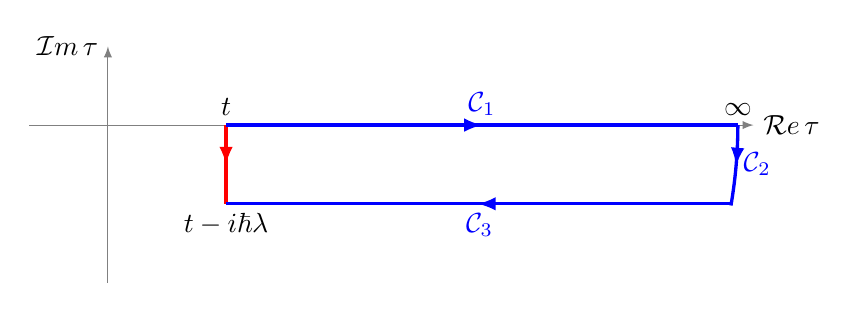
\begin{tikzpicture}
				\draw[-latex,gray] (-1,0) -- (8.2,0);
				\draw[-latex,gray] (0,-2) -- (0,1);
				\begin{scope}[very thick,decoration={ % See https://tex.stackexchange.com/questions/3161/tikz-how-to-draw-an-arrow-in-the-middle-of-the-line/3172#3172
						markings,
						mark=at position 0.5 with {\arrow{latex}}}
					]
					\draw[postaction={decorate},red] (1.5,0) -- (1.5,-1);
					\draw[postaction={decorate},blue] (1.5,0)--(8,0);
					\draw[postaction={decorate},shift={(8,0)},blue] (0,0) arc (0:-9.8:6);
					\draw[postaction={decorate},blue] (7.9,-1)--(1.5,-1);
				\end{scope}
				\node[above] at (1.5,0) {$t$};
				\node[below] at (1.5,-1) {$t-i\hbar\lambda$};
				\node[above] at (8,0) {$\infty$};
				\node[right] at (8.2,0) {$\mathop{\mathcal{R}e}\tau$};
				\node[left] at (0,1) {$\mathop{\mathcal{I}m}\tau$};

				\node[above] at (4.75,0) {\color{blue}$\mathcal{C}_1$};
				\node[right] at (7.95,-0.5) {\color{blue}$\mathcal{C}_2$};
				\node[below] at (4.72,-1) {\color{blue}$\mathcal{C}_3$};
			\end{tikzpicture}
			\caption{{\bf Complex-$\tau$ Plane}. Cauchy's theorem ensures that the integration along red path can be replaced by the integration along the blue path $\mathcal{C}_1+\mathcal{C}_2+\mathcal{C}_3$, with the contribution over $\mathcal{C}_2$ being vanishing.}
			\label{fig:contour}
		\end{figure}
		
		\noindent Including the non-vanishing contribution from the contour $\mathcal{C}_1$ and $\mathcal{C}_2$, we have, the conductivity tensor,
		\begin{align}
			\sigma_{\gamma\varphi}(\omega)&=\lim_{s \rightarrow0^+}\int_0^\infty\dd t\,e^{i\varpi t}\int_0^\beta\dd\lambda\,\langle J(\delta\gamma,t-i\hbar\lambda)J(\delta\varphi)\rangle=\dfrac{-1}{i\hbar}\lim_{s \rightarrow0^+}\int_0^\infty\dd t\,e^{i\varpi t}\int_t^{t-i\hbar\beta}\dd\tau\,\langle J(\delta\gamma,\tau)J(\delta\varphi)\rangle\nonumber\\
			&=\dfrac{-1}{i\hbar}\lim_{s \rightarrow0^+}\int_0^\infty\dd t\,e^{i\varpi t}\int_t^\infty\dd t'\bigg(\langle J(\delta\gamma,t')J(\delta\varphi)\rangle-\langle J(\delta\gamma,t-i\hbar\beta)J(\delta\varphi\rangle)\bigg)\nonumber\\
			&=\dfrac{-1}{i\hbar}\lim_{s \rightarrow0^+}\int_0^\infty\dd t\,e^{i\varpi t}\int_t^\infty\dd t'\,\mathop{\mathrm{Tr}}\bigg\{\rho_0\bigg(J(\delta\gamma,t')J(\delta\varphi)-e^{\beta H_0}J(\delta\gamma,t)e^{-\beta H_0}J(\delta\varphi)\bigg)\bigg\}\nonumber\\
			&=\dfrac{-1}{i\hbar}\lim_{s \rightarrow0^+}\int_0^\infty\dd t\,e^{i\varpi t}\int_t^\infty\dd t'\,\mathop{\mathrm{Tr}}\bigg\{\rho_0\bigg(J(\delta\gamma,t')J(\delta\varphi)-J(\delta\varphi)J(\delta\gamma,t)\bigg)\bigg\}\nonumber\\
			&=\dfrac{-1}{i\hbar}\lim_{s \rightarrow0^+}\int_0^\infty\dd t\,e^{i\varpi t}\int_t^\infty\dd t'\,\langle[J(\delta\gamma,t'),J(\delta\varphi)]\rangle.\label{2.2.8}
		\end{align}
		Integration by parts, we get
		\begin{align}
			\sigma_{\gamma\varphi}(\omega)&=\lim_{s \rightarrow0^+}\dfrac{1}{\hbar\varpi}\left\{\left.e^{i\varpi t}\int_t^\infty\dd t'\,\langle[J(\delta\gamma,t'),J(\delta\varphi)]\rangle\right|_0^\infty-\int_0^\infty\dd t\, e^{i\varpi t}\dfrac{\dd}{\dd t}\int_t^\infty\dd t'\,\langle[J(\delta\gamma,t'),J(\delta\varphi)]\rangle\right\}\nonumber\\
			&=\lim_{s \rightarrow0^+}\dfrac{-1}{i\varpi}\left\{\dfrac{-1}{i\hbar}\int_0^\infty\dd t\,\langle[J(\delta\gamma,t),J(\delta\varphi)]\rangle+\dfrac{1}{i\hbar}\int_0^\infty\dd t\,e^{i\varpi t}\langle[J(\delta\gamma,t),J(\delta\varphi)]\rangle\right\}\nonumber\\
			&\equiv\lim_{s \rightarrow0^+}\dfrac{-1}{i\varpi}\bigg\{\Sigma_{\gamma\varphi}(\omega)-\Sigma_{\gamma\varphi}(0)\bigg\}\label{2.2.9}
		\end{align}
		with the familiar response function $\Sigma_{\gamma\varphi}(\omega)$ for the \emph{total} current.\par
		\indent Again if we try to go back to the system with quadratic dispersion relation up to linear response, we have to prove that $-\chi_{\gamma\varphi}(0)$ is indeed the diamagnetic part of contribution. In fact, by taking similar steps as \eqref{1.4.2} and working in momentum space, we get
		\begin{equation}\label{2.2.10}
			-\Sigma_{\gamma\varphi}(\bm{q},0)=\cdots=-\dfrac{1}{V}\sum_{m,n}(f_m-f_n)\dfrac{\langle m|J_\gamma^{(1)}(\bm{q})|n\rangle\langle n|J_\varphi^{(1)}(\bm{-q})|m\rangle}{\varepsilon_m-\varepsilon_n}.
		\end{equation}
		And f-sum rule immediately tells
		\begin{equation}\label{2.2.11}
			-\Sigma_{\gamma\varphi}(\bm{q},0)=\dfrac{nq^2}{m}\delta_{\gamma\varphi},
		\end{equation}
		matching perfectly with the diamagnetic part.

	\subsection{Matsubara Green Function of Imaginary-frequencies}
		Since the response function $\Sigma_{\gamma\varphi}(\omega)$ (or paramagnetic response function $\chi_{\gamma\varphi}(\omega)$) contains a kernel of retarded Green function $G^R_{J_\gamma J_\varphi}(\omega)$, we can also evaluate it with the help of Matsubara Green function (of current operators) on imaginary-frequency domain
		\begin{equation*}
			\mathcal{G}_{J_\gamma J_\varphi}(i\omega_n)\equiv\int_0^\beta\dd\tau\,e^{i\omega_n\tau}\mathcal{G}_{J_\gamma J_\varphi}(\tau)\equiv\int_0^\beta\dd\tau\,e^{i\omega_n\tau}(-1)\langle\mathcal{T}_\tau J(\delta\gamma,\tau) J(\delta\varphi)\rangle=-\int_0^\beta\dd\tau\,e^{i\omega_n\tau}\langle J(\delta\gamma,\tau) J(\delta\varphi)\rangle.
		\end{equation*}
		and analytical continuation
		\begin{equation*}
			G^R_{J_\gamma J_\varphi}(\omega)=\left.\mathcal{G}_{J_\gamma J_\varphi}(i\omega_n)\right|_{i\omega_n \rightarrow i\omega+0^+}.
		\end{equation*}
		The imaginary-time order is removed here just because the integration is performed on $[0,\beta)$ (essentially this comes from the (anti-)periodicity of the Matsubara Green function for boson (fermion) $\mathcal{G}(\tau)\equiv\mp\mathcal{G}(\tau+i\hbar\beta)$). This approach is gauranteed by the Lehmann spectral representation of their definition \cite{abrikosov2012methods,mahanmany}. For instance, Scalapino \textit{et al.} \cite{scalapino1993insulator} employ such method to study the fast and slow limits for metals, insulators, and superconductors.


\section{Appendix}
	\subsection{f-sum Rule}
		In this section, we will give a proof of the identity \eqref{1.4.6} used in the main text. Let me quote it here again
		\begin{Theorem}[(f-sum Rule)]
			\begin{equation}\label{a.1.1}
				\sum_{m,n}(f_m-f_n)\dfrac{\langle m|J^{(1)}_\alpha(\bm{q})|n\rangle\langle n|J^{(1)}_\beta(-\bm{q})|m\rangle}{\varepsilon_{mn}}=-\dfrac{Nq^2}{m}\delta_{\alpha\beta}.
			\end{equation}
		\end{Theorem}
		\begin{Proof}
			Relabling the states, we have, equivalently
			\begin{align}
				\text{LHS}&=\sum_{m,n}f_m\dfrac{\langle m|J^{(1)}_\alpha(\bm{q})|n\rangle\langle n|J^{(1)}_\beta(-\bm{q})|m\rangle+\langle m|J^{(1)}_\beta(-\bm{q})|n\rangle\langle n|J^{(1)}_\alpha(\bm{q})|m\rangle}{\varepsilon_m-\varepsilon_n}\nonumber\\
				&=\sum_{m,n}f_m\dfrac{\frac{-1}{\hbar q^\alpha}(\varepsilon_m-\varepsilon_n)}{\varepsilon_m-\varepsilon_n}\bigg(\langle m|Q^{(1)}(\bm{q})|n\rangle\langle n|J^{(1)}_\beta(-\bm{q})|m\rangle-\langle m|J^{(1)}_\beta(-\bm{q})|n\rangle\langle n|Q^{(1)}(\bm{q})|m\rangle\bigg)\nonumber\\
				&=\dfrac{-1}{\hbar q^\alpha}\sum_m f_m\langle m|[Q(\bm{q}),J_\beta^{(1)}(-\bm{q})]|m\rangle,\label{a.1.2}
			\end{align}
			where in the second line, we make use of the momentum space charge conservation law
			\begin{equation*}
				\dfrac{\dd Q(\bm{q},t)}{\dd t}\equiv\dfrac{1}{i\hbar}[Q(\bm{q}),h]=-\dfrac{i}{\hbar}\bm{q}\cdot\bm{J}(\bm{q})
				%\dfrac{1}{i\hbar}\left[e^{-\frac i\hbar\bm{q}\cdot\hat{\bm{r}}},\dfrac{\hat p^2}{2m}\right]=\dfrac{1}{2mi\hbar}[e^{-\frac i\hbar\bm{q}\cdot\hat{\bm{r}}},\hat p^\alpha]\hat p_\alpha=\dfrac{1}{2mi\hbar}e^{-\frac i\hbar\bm{q}\cdot\hat{\bm{r}}}q^\alpha\hat p_\alpha\equiv Q(\bm{q})\dfrac{\bm{q}\cdot\hat{\bm{p}}}{2mi\hbar}=
			\end{equation*}
			and take the quantum average over states $\langle m|$ and $|n\rangle$
			\begin{equation}\label{a.1.3}
				(\varepsilon_n-\varepsilon_m)\langle m|Q(\bm{q})|n\rangle=q^\alpha\langle m|J_\alpha(\bm{q})|n\rangle
			\end{equation}
			to replace the average of current operators. The commutator in \eqref{a.1.2} can be calculated by inserting the first quantized charge currents and charge densities (do not get confused with the charge $q$ and momentum $q_\alpha$...)
			\begin{equation}\label{a.1.4}
				[Q(\bm{q}),J_\beta(-\bm{q})]=\left[q e^{-\frac i\hbar\bm{q}\cdot\hat{\bm{r}}},\dfrac{q}{2m}(\hat p_\beta e^{\frac i\hbar\bm{q}\cdot\hat{\bm{r}}}+e^{\frac i\hbar\bm{q}\cdot\hat{\bm{r}}}\hat p_\beta)\right]=\dfrac{q^2}{2m}\bigg[(e^{-\frac i\hbar\bm{q}\cdot\hat{\bm{r}}}\hat p_\beta e^{\frac i\hbar\bm{q}\cdot\hat{\bm{r}}}+\hat p_\beta)-(\hat p_\beta+e^{\frac i\hbar\bm{q}\cdot\hat{\bm{r}}}\hat p_\beta e^{-\frac i\hbar\bm{q}\cdot\hat{\bm{r}}})\bigg]=\dfrac{q^2\cdot q_\alpha}{m}\delta_{\alpha\beta}.
			\end{equation}
			Thus we have
			\begin{equation*}
				\text{LHS}=-\dfrac{q^2}{m}\delta_{\alpha\beta}\sum_m f_m=-\dfrac{Nq^2}{m}\delta_{\alpha\beta}=\text{RHS}.
			\end{equation*}
		\end{Proof}

		The foundamental form of the f-sum rule (see in \cite{anderson1958coherent}) with approach 1 can also be used to derive the much more familiar result:
		\begin{Corollary}[(Integration Form of f-sum Rule)]
			\begin{equation}\label{a.1.5}
				\dfrac{1}{2\pi}\int_{-\infty}^\infty\dd\omega\,\sigma_{\gamma\varphi}(\omega)=\dfrac{nq^2}{2m}\delta_{\gamma\varphi}
			\end{equation}
		\end{Corollary}
		\begin{Proof}
			Taking the form of conductivity tensor as \eqref{2.2.1} and change the order of integration, we have
			\begin{align*}
				\text{LHS}&=\lim_{s \rightarrow0^+}\dfrac{1}{2\pi}\int\dd\omega\,\dfrac{1}{i\hbar}\int_0^\infty\dd t\,\langle[J(\delta\gamma,t),Q(\varphi)]\rangle_0e^{i\varpi t}=\dfrac{1}{i\hbar}\int_{-\infty}^\infty\dd t\,\theta(t)\langle[J(\delta\gamma,t),Q(\varphi)]\rangle_0 \delta(t)\\
				&=\dfrac{1}{2i\hbar}\langle[J(\delta\gamma),Q(\varphi)]\rangle_0=\dfrac{nq^2}{2m}\delta_{\gamma\varphi},
			\end{align*}
			where in first line we take the Heaviside theta function $\theta(0)=\frac{1}{2}$ and in the second line we insert the equivalence with the diamangetic part \eqref{2.2.7}.
		\end{Proof}

\bibliography{hxd}
\bibliographystyle{apsrev} % apsrev is format for PRL of APS
\end{document}